%_____________________________________________________________________________________________ 
% LATEX Template: Department of Computer Engineering BTech Project Report
% Main Report
% Sun Apr 7 20:40:00 IST 2024
% 
%_____________________________________________________________________________________________ 

\documentclass[a4paper,14pt,onecolumn]{report}

%_____________________________________________________________________________________________ 
% Inclusion of Required Packages
%_____________________________________________________________________________________________ 
\usepackage[dvips]{graphics}
\usepackage{color}
\usepackage{epsfig}
%_____________________________________________________________________________________________ 
% Page Layout
%_____________________________________________________________________________________________ 
\setlength{\textwidth}{6.27in}
\setlength{\textheight}{9.69in}
\setlength{\topmargin}{0.0in}
\setlength{\oddsidemargin}{0.0in}			% Customisable
\setlength{\headheight}{0.0in}
\setlength{\headsep}{0.0in}
\setlength{\topskip}{0.0in}
%_____________________________________________________________________________________________ 
% Font Definition
%_____________________________________________________________________________________________ 
\fontencoding{T1}		% Font specification : Times New Roman, Bold, Normal, 18
\fontfamily{cmr}		% Roman
\fontseries{m}			% Medium
\fontshape{n}			% Upright
\fontsize{14pt}{5}		
\linespread{1.5}		% Vertical spacing between lines
\selectfont			% Select the specified font
%_____________________________________________________________________________________________ 
% Main report starts here
%_____________________________________________________________________________________________ 

\begin{document}	% Start of Report
	%_____________________________________________________________________________________________ 
	\pagestyle{empty}
	\begin{titlepage}
		\begin{center}
			\LARGE{\bf{RETAIL E-COMMERCE PRICE TRACKER\\}}	% LARGE = 17.28
			\vspace{10pt}
			\Large{\bf{A Project Report\\}}		% Large = 14.40
			\Large{\em{Submitted by\\}}
			\begin{table}[htbp]
				\begin{center}
					\begin{tabular}{ l c c l }
						\Large\bf{Ketan Kale} & & & \Large\bf{112103064} \\
						\Large\bf{Nikhil Kokale} & & & \Large\bf{112103072} \\
						\Large\bf{Atharva Lonhari} & & & \Large\bf{112103079} \\[0.3cm] 
						
					\end{tabular}
				\end{center}
			\end{table}
			\Large{\em{of\\}}
			\LARGE{\bf{TY  (Computer Engineering)\\}}% Mention only appropriate degree.
			\vspace{20pt}
			%names of advisors
			\Large{Under the guidance of\\ }
			\Large{\bf{Dr. Tanuja R. Pattanshetti \\ }\\}
			\Large{COEP Technological University\\}
			\vspace{10pt}
			%coep logo added
			\begin{figure}[h]
				\centering
				\includegraphics[width=3cm,height=3cm]{collegelogo.png}
			\end{figure}
			\Large{\bf{DEPARTMENT OF COMPUTER ENGINEERING\\ 
					COEP Technological University}}
			\vfill
			\large{April, 2024}
		\end{center}
	\end{titlepage}
	
	\thispagestyle{empty}
	\linespread{2}
	\begin{center}			% LARGE = 18
		\Large{\bf{DEPARTMENT OF COMPUTER ENGINEERING\\ 
				COEP Technological University\\}}	
	\end{center}
	
	\vspace{20pt}			% Vertical space between dept name and ``certi''
	
	\begin{center}
		\Large{\bf{CERTIFICATE\\}}
	\end{center}
	
	\vspace{20pt}
	
	\linespread{2}			% Double spacing between lines
	\selectfont
	\large{
		Certified that this project, titled ``RETAIL E-COMMERCE PRICE TRACKER''
		has been successfully completed by \\ 
		\begin{table}[htbp]
			\begin{center}
				\begin{tabular}{ l c c l }
					\Large\bf{Ketan Kale} & & & \Large\bf{112103064} \\
					\Large\bf{Nikhil Kokale} & & & \Large\bf{112103072} \\
					\Large\bf{Atharva Lonhari} & & & \Large\bf{112103079} \\[0.3cm]
					
				\end{tabular}
			\end{center}
		\end{table} \\
		and is approved for the fulfilment of the requirements of 
		``Software Engineering Mini Project- Stage II''.
	}
	
	\vspace{100pt}
	
	\begin{center}		% Horizontal spacing used to keep the signatures in columns at the ends of
		% lines
		
		\hspace{\stretch{1}}SIGNATURE\\
		\normalsize{\bf{\hspace{\stretch{1}}\Large{\bf{Dr. Tanuja R. Pattanshetti \\ }\\}\\
				\hspace{\stretch{1}}Project Guide}\\
			\hspace{\stretch{1}}Department of Computer Engineering\\
			\hspace{\stretch{1}}COEP Technological University,\\
			\hspace{\stretch{1}}Shivajinagar, Pune - 5.}
	\end{center}
	
	\begin{abstract}
		%\addcontentsline{toc}{chapter}{Abstract}	% This makes sure abstract is included in contents.
		The Retail E-Commerce Price Tracker project aims to develop a comprehensive web application that empowers users to track and compare prices of electronic items across multiple online retailers. In a dynamic and competitive online marketplace, consumers often face challenges in finding the best deals and making informed purchasing decisions. The Retail E-Commerce Price Tracker addresses this need by leveraging web scraping techniques to collect real-time pricing data from various online retailers and presenting it through a user-friendly interface.
		\\
		The project methodology involves thorough requirements analysis, technology selection, system design, implementation, and testing. Key features of the application include price comparison, price tracking with alerts, deal discovery, historical price analysis, product research, budget planning, and market analysis.
		\\
		Through the implementation of the Retail E-Commerce Price Tracker application, users can efficiently navigate the electronic marketplace, compare prices, monitor price trends, and receive alerts on price drops, ultimately enabling them to make informed purchasing decisions and maximize savings. The project contributes to enhancing the overall shopping experience for consumers and provides valuable insights for retailers and industry analysts.
		\\
		The outcomes of the project highlight the effectiveness of the Retail E-Commerce Price Tracker application in addressing the challenges faced by consumers in the electronic marketplace. By providing a centralized platform for price comparison and analysis, the application empowers users to make informed decisions and optimize their shopping experience.
	\end{abstract}
	
	
	% \maketitle
	\tableofcontents
	\listoffigures 
	
	
	
	\mainmatter
	
	
	
	\titleformat{\chapter}
	\chapter{Synopsis}
	
	\section{Project Title}
	\begin{itemize}
		RETAIL E-COMMERCE PRICE TRACKER 
	\end{itemize}
	
	
	\section{Internal Guide}
	\begin{itemize}
		Dr. Tanuja R. Pattanshetti
	\end{itemize}
	
	
	\section{Problem Statement}
	\label{sec:problem}
	\begin{itemize}
		The Electronic Price Tracker project addresses the need for a centralized platform to track and compare prices of electronic items across multiple online retailers. It aims to provide users with real-time pricing information and personalized alerts on price drops, enhancing their ability to make informed purchasing decisions and maximize savings. The project seeks to empower consumers in navigating the electronic marketplace efficiently and confidently, ensuring they secure the best possible prices for their desired products. 
	\end{itemize}
	
	\section{Plan of Project Execution}
	\begin{left}
		\begin{tabular}{p{4cm} | p{2cm} | p{2cm} | p{1.5cm} | p{1cm}} 
			Task & Start Date & End Date & Duration & Resources \\ [0.5ex] 
			\hline
			
			Problem statement finalization & 08-Jan-24 & 15-Jan-24 & 8 & Atharva,Ketan,Nikhil
			\\ 
			\hline
			Project Plan & 16-Jan-24 & 31-Jan-24 & 16 & Atharva 
			\\
			\hline
			Requirement Analysis & 01-Feb-24 & 05-Feb-24 & 5 & Ketan,Atharva \\
			\hline
			Functional Flow and Screens Identification & 06-Feb-24 & 09-Feb-24 & 4 & Nikhil,Atharva
			\\
			\hline
			Creating Mocks for each of the Screens Identified & 10-Feb-24 & 13-Feb-24 & 4 & Ketan
			\\
			\hline
			Web Scraping POC & 13-Feb-24 & 18-Feb-24 & 6 & Nikhil
			\\
			\hline
			Database Modelling & 19-Feb-24 & 29-Feb-24 & 10 & Atharva
			\\
			\hline
			Data population using Web scraping & 01-Mar-24 & 10-Mar-24 & 10 & Atharva,Nikhil
			\\
			\hline
			Price comparision functionality & 11-Mar-24 & 20-Mar-24 & 10 & Atharva,Ketan,Nikhil
			\\
			\hline
			Frontend & 21-Mar-24 & 31-Mar-24 & 10 & Ketan,Nikhil
			\\
			\hline
			Testing & 01-Apr-24 & 10-Apr-24 & 10 & Atharva,Ketan,Nikhil
			\\
			\hline
			Documentation and project report & 11-Apr-24 & 15-Apr-24 & 5 & Atharva,Ketan,Nikhil\\[1ex] 
			\hline
		\end{tabular}
	\end{left}
	
	
	\chapter{Problem Definition and scope}
	\section{Problem Definition}
	\subsection{Goals and objectives}  
	Goal and Objectives: 
	\begin{itemize}
		\item Goals
		\begin{itemize}
			\item Develop a software solution that empowers consumers to find the best
			product deals and save money on their online purchases.
		\end{itemize}
		\item Objectives
		\begin{itemize}
			\item \textbf{Aggregate product pricing data:} Collect and organize product pricing
			information from a wide range of online retailers in a timely and accurate
			manner.
			\item \textbf{Enable comprehensive price comparison:}Develop algorithms to compare
			prices across retailers.
			\item \textbf{Offer personalized deal recommendations:}Recommend the best deal to
			each user based on their customizable preferences and priorities.
			\item \textbf{Provide price drop alerts:}Monitor price changes for specific products and
			send timely alerts to users when desired price drops occur.
			`           \item \textbf{Deliver a user-friendly interface:}Create an intuitive and accessible user
			interface that facilitates easy product search, comparison, etc.
		\end{itemize}
	\end{itemize}
	
	\subsection{Statement of scope} 
	\begin{itemize}  
		\item	\textbf{Target Products:} Laptops, Smartphones, T.V.s, Refrigerators
		\item \textbf{Target Websites:} Vijay Sales, Croma, Reliance Digital, Flipkart
		\item \textbf{Target Audience:}  This application is ideal for consumers who are looking to
		save money on their electronics purchases. It will be particularly beneficial
		for individuals who frequently buy or research electronic products
	\end{itemize}
	
	\section{Software context} 
	\begin{itemize}
		The Retail E-Commerce Price Tracker project operates within the context of web application development and data aggregation. It involves the integration of web scraping techniques to gather real-time pricing information from various online retailers. The project will utilize technologies such as HTML, CSS, and JavaScript for front-end development to create a user-friendly interface. On the back end, the application will be developed using programming languages like Python, along with frameworks such as Flask, to handle data processing, storage, and user authentication.
		\\
		Additionally, the project may leverage libraries and tools specific to web scraping, such as BeautifulSoup, to extract data efficiently from retailer websites. Database management systems like MySQL may be employed to store and manage the collected data.
		\\
		Overall, the software context of the Electronic Price Tracker project encompasses web development, data aggregation, database management, and cloud computing technologies, all aimed at creating a robust and efficient platform for tracking and comparing electronic item prices across online retailers.
	\end{itemize}
	\section{Major Constraints}
	\begin{itemize}
		\item \textbf{Data acquisition}
		\begin{itemize}
			\item \textbf{Website structure and its changes:} Adapting to variations in website layouts and data formats.
			\item \textbf{Volume of data:} Handling large number of websites.
			\item \textbf{Ethical Scraping:} The techniques must comply with website terms of service and keep in mind data privacy regulations.
		\end{itemize}
		\item \textbf{Client-side constraints}
		\begin{itemize}
			\item \textbf{Offline users:} Users not being logged in to the application.
			\item \textbf{Synchronization of Data:} We need to ensure the consistency of client-side and server-side data and ensure they are synchronized.
		\end{itemize}
		\item \textbf{Data processing}
		\begin{itemize}
			\item \textbf{Optimization of performance:} We need to process large datasets effectively without compromising speed.
		\end{itemize}
		
	\end{itemize}
	
	\section{Outcome}
	The primary outcome of the Retail E-Commerce Price Tracker project is the successful development and deployment of a comprehensive web application that empowers users to track and compare prices of electronic items across multiple online retailers. Key components of the outcome include:
	\begin{itemize}
		\item \textbf{User-Friendly Interface:} A user-friendly interface that enables users to easily navigate the application, search for electronic items, and compare prices from various online retailers. The interface is intuitive and visually appealing.
		
		\item \textbf{Real-Time Pricing Information:} The application provides users with up-to-date pricing information from multiple online retailers, ensuring accuracy and reliability. Data collected through web scraping techniques is regularly updated to reflect changes in pricing.
		
		\item \textbf{Personalized Alerts:} The ability for users to set up personalized alerts for price drops on specific electronic items of interest. These alerts are timely, notifying users via email when prices decrease on selected items.
		
		\item \textbf{Efficient Data Aggregation:} Efficient data aggregation and processing mechanisms to collect pricing information from various online retailers seamlessly.
		
		\item \textbf{Enhanced User Experience:} The outcome results in an enhanced user experience, enabling users to make informed purchasing decisions and maximize savings in the electronic marketplace.
		
	\end{itemize}
	
	\section{Applications}
	\begin{itemize}
		\item \textbf{Comparison Shopping:} The Retail E-Commerce Price Tracker application enables users to compare prices of electronic items across multiple online retailers, facilitating informed purchasing decisions and ensuring they obtain the best possible prices.
		
		\item \textbf{Price Tracking and Alerts:} Users can track the prices of specific electronic items over time and set up personalized alerts for price drops. This feature helps users stay informed about cost-saving opportunities and capitalize on favorable price changes.
		
		\item \textbf{Budget Planning:} The application can be used as a budget planning tool, allowing users to monitor prices of electronic items and plan their purchases accordingly. By tracking price trends and setting budget thresholds, users can optimize their spending and maximize savings.
		
		\item \textbf{Deal Hunting:} Users can leverage the application to hunt for deals and discounts on electronic items, taking advantage of price drops and promotional offers from various online retailers. This can lead to significant cost savings on desired products.
		
		\item \textbf{Market Analysis:} The aggregated pricing data collected by the application can be utilized for market analysis purposes. Retailers and industry analysts can analyze pricing trends, demand patterns, and competitive landscape to gain insights into market dynamics and consumer behavior.
		
		\item \textbf{Price Monitoring for Retailers:} Retailers can use the application to monitor prices of their own products as well as competitors' prices, enabling them to adjust pricing strategies and stay competitive in the market.
		
		\item \textbf{Educational Purposes:} The application can be used for educational purposes, such as teaching students about web scraping techniques, data aggregation, and market analysis in the context of e-commerce and online retailing.
	\end{itemize}
	
	\section{Software Resources Required}
	\begin{enumerate}
		\item \textbf{Database Management System (DBMS):} A relational database management system (RDBMS) such as MySQL is required to store and manage the application's data, including pricing information and user accounts. 
		
		\item \textbf{Web Framework:} A web framework is necessary for developing the backend logic of the Retail E-Commerce Price Tracker application.
		
		\item \textbf{Web Scraping Tools:} Software tools and libraries for web scraping are required to collect real-time pricing data from various online retailers.
		
		\item \textbf{Programming Languages:} Programming languages such as Python, JavaScript, HTML, CSS, and SQL are essential for developing different components of the Retail E-Commerce Price Tracker application, including backend logic, frontend interfaces, and database queries.
		
		\item \textbf{Version Control System:} Version control software such as Git is necessary for managing the application's source code, tracking changes, and collaborating with team members.
	\end{enumerate}
	\newpage
	\chapter{Project Plan}
	\section{Project Schedule}  
	\subsection{Gantt Chart}  
	\includegraphics[width=500pt]{GanttChart.png}
	
	\chapter{Software requirement specification}
	
	\section{Introduction}
	\subsection{Use-cases}
	\begin{itemize}
		\item \textbf{Price Comparison:} Users compare prices of electronic items from multiple retailers.
		\item \textbf{Price Tracking:} Users track item prices and receive alerts for drops.
		\item \textbf{Deal Discovery:} Users find discounts and promotions on electronics.
		\item \textbf{Historical Price Analysis:} Users review past prices to gauge trends.
		\item \textbf{Product Research:} Users compare specs, reviews, and prices.
		\item \textbf{Budget Planning:} Users set budgets and monitor prices accordingly.
		\item \textbf{Market Analysis:} Retailers analyze pricing trends for competitiveness.
	\end{itemize}
	
	\subsection{Use Case View}
	Use Case Diagram:
	\begin{center}
		\begin{figure}[!htbp]
			\centering
			\fbox{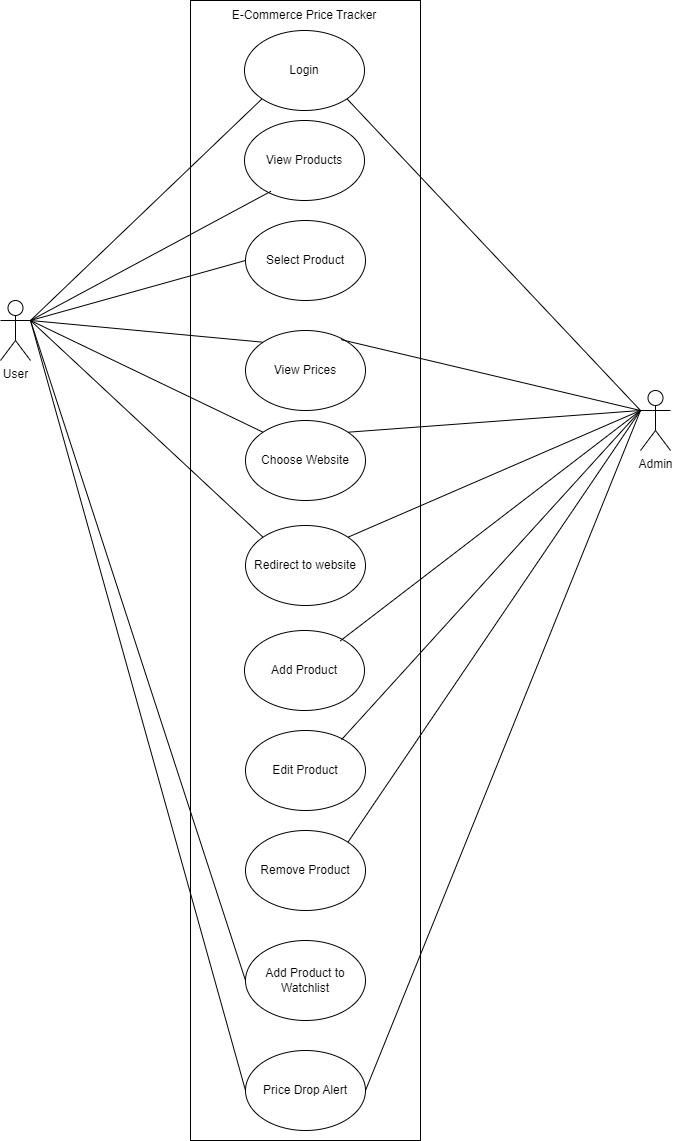
\includegraphics[width=\textwidth]{UseCaseDiagram.drawio.png}}
			\caption{Use case diagram}
			\label{fig:usecase}
		\end{figure}
	\end{center}  
	
	\section{Data Model and Description}  
	\subsection{Data objects and Relationships}
	\begin{itemize}
		\item \textbf{User:}Represents a registered user of the Retail E-Commerce Price Tracker application. Users can log in, authenticate, and access personalized features such as price tracking and watchlists.
		\item \textbf{Product:}Represents an electronic item available for tracking and comparison within the application. Product details provide users with information about the items they are interested in purchasing.
		\item \textbf{Price:}Stores pricing information for different products from various online retailers. Prices are regularly updated through web scraping techniques to provide users with real-time pricing data.
		\item \textbf{Watchlist:}Allows users to monitor specific products for price drops. Users can add products to their watchlists and receive alerts when prices fall below their specified target prices.
	\end{itemize}
	\clearpage
	Entity Relationship Diagram:
	\begin{center}
		\begin{figure}[!htbp]
			\centering
			\fbox{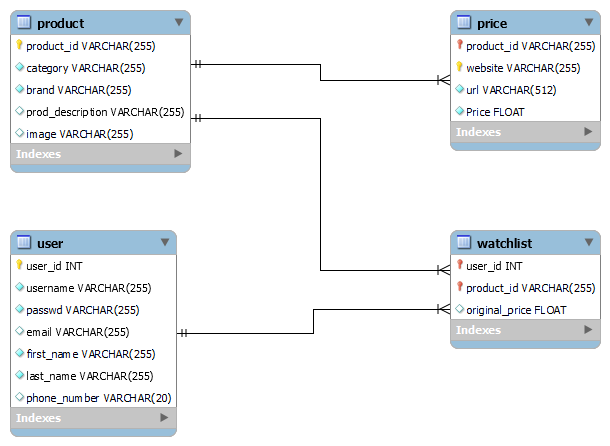
\includegraphics[width=500pt]{ERD.png}}
			\caption{Entity Relationship diagram}
			\label{fig:EntityRelationDiagram}
		\end{figure}
	\end{center} 
	
	
	
	\section{Functional Model and Description}   
	\subsection{Data Flow Diagram}  
	\newpage
	\subsubsection{Level 0 Data Flow Diagram}
	\begin{center}
		\begin{figure}[!htbp]
			\centering
			\fbox{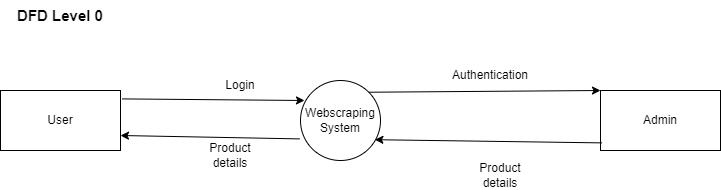
\includegraphics[width=\textwidth]{DFD_Level0.drawio.png}}
			\caption{DFD Level0}
			\label{fig:DFDLevel0}
		\end{figure}
	\end{center} 
	\subsubsection{Level 1 Data Flow Diagram}
	\begin{center}
		\begin{figure}[!htbp]
			\centering
			\fbox{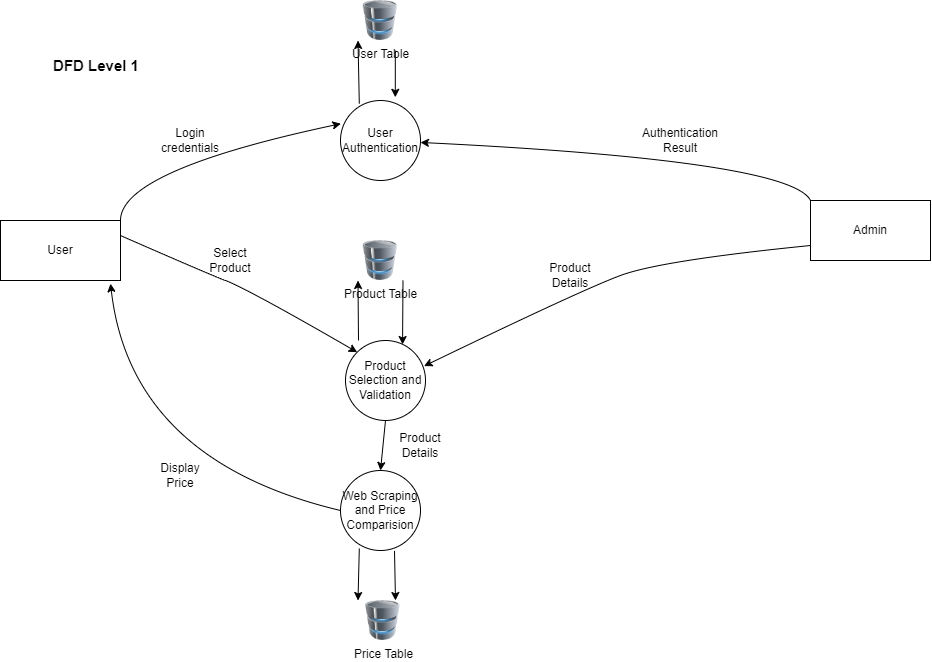
\includegraphics[width=\textwidth]{DFD_Level1.drawio.png}}
			\caption{DFDLevel1}
			\label{fig:DFDLevel1}
		\end{figure}
	\end{center} 
	\subsubsection{Level 2 Data Flow Diagram}
	\begin{center}
		\begin{figure}[!htbp]
			\centering
			\fbox{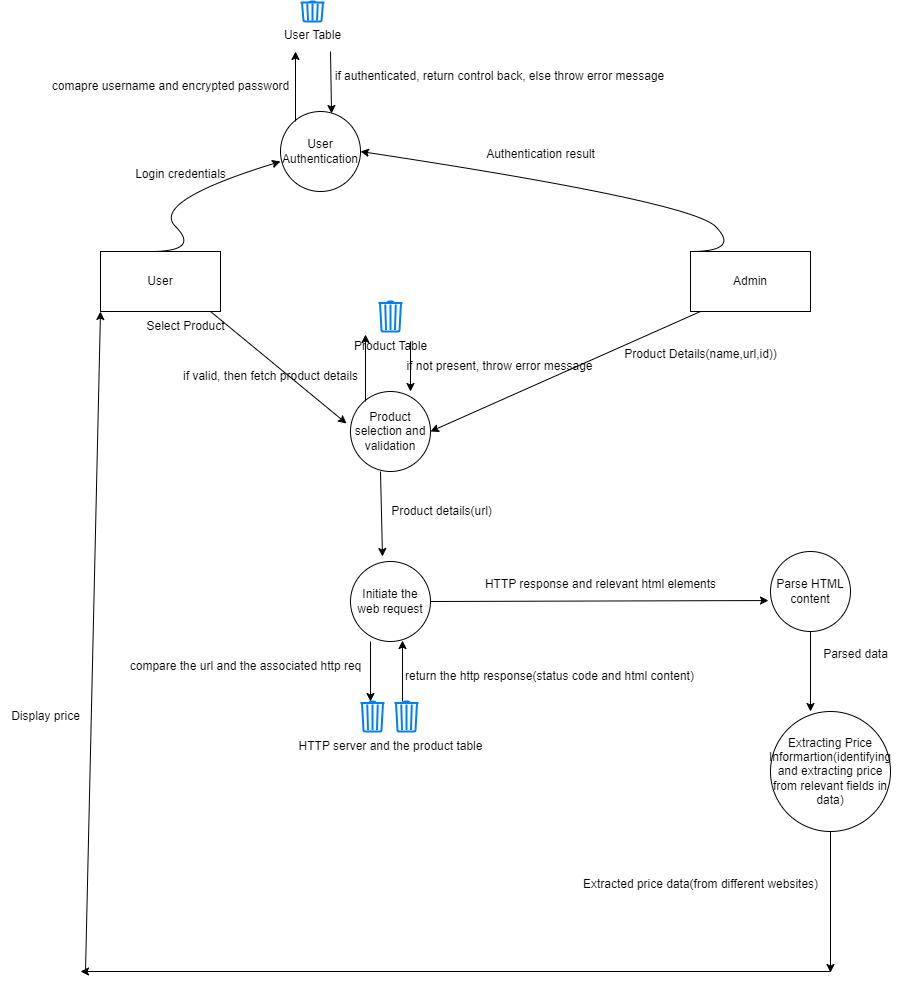
\includegraphics[width=\textwidth]{DFD_Level2.drawio.png}}
			\caption{DFDLevel2}
			\label{fig:DFDLevel2}
		\end{figure}
	\end{center} 
	
	\subsection{Description of functions}  
	
	
	
	
	
	\subsection{Activity Diagram:}
	\begin{itemize}
		\item	The Activity diagram represents the steps taken.
	\end{itemize} 
	\begin{center}
		\begin{figure}[!htbp]
			\centering
			\fbox{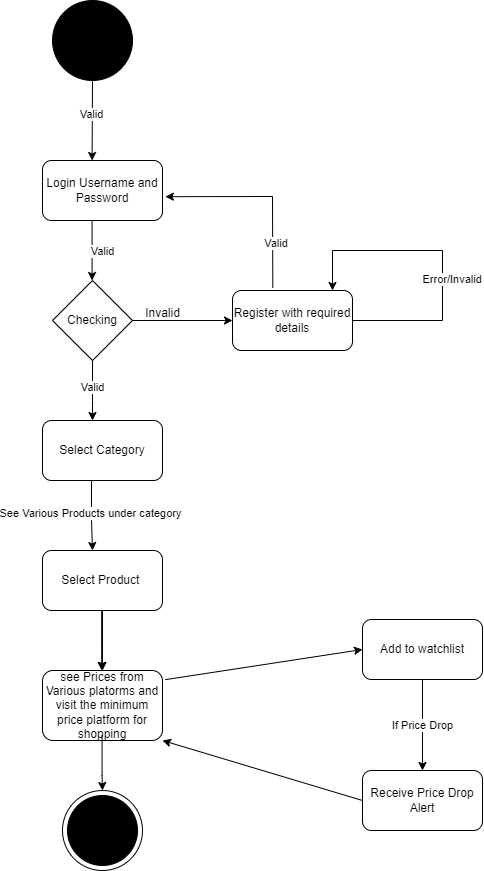
\includegraphics[height=430pt]{ActivityDiagram.drawio.png}}
			\caption{Activity diagram}
			\label{fig:act-dig}
		\end{figure}
	\end{center}  
	
	
	\subsection{Non Functional Requirements:}
	\subsubsection{Performance Requirements}
	\begin{itemize}
		\item \textbf{Response Time:} The system should respond to user actions (login, product selection, price comparison) within a reasonable time frame.
		\item \textbf{Scalability:} The system should be able to handle an increasing number of users and products without a significant decrease in performance. This involves efficient use of server resources and possibly implementing load balancing techniques.
		\item \textbf{Concurrency:} The system should support multiple users accessing and interacting with the application simultaneously without experiencing performance degradation. This includes handling concurrent requests for web scraping data from multiple websites.
		\item \textbf{Error Handling:} The system should handle errors gracefully, providing meaningful error messages to users and logging errors for system administrators to troubleshoot performance issues.
		\item \textbf{Database Performance:} Ensure efficient database performance for storing user information, product data, and price comparisons. This includes optimizing database queries and indexing for faster data retrieval.
	\end{itemize} 
	\subsubsection{Safety and Security Requirements:}
	\begin{itemize}
		\item \textbf{Data Privacy:} Ensure that user login credentials, personal information, and transaction details are securely stored and encrypted to prevent unauthorized access or data breaches.
		\item \textbf{Input Validation:} Implement input validation ensure that user inputs are safe and free from malicious inputs.
		\item \textbf{Content Integrity:} Verify the integrity of scraped content to ensure that prices and product information obtained from external websites are accurate and reliable, minimizing the risk of misleading or fraudulent data.
	\end{itemize}
	
	
	\subsection{Design Constraints}	
	\begin{itemize}
		\item \textbf{Data acquisition}
		\begin{itemize}
			\item \textbf{Website structure and its changes:} Adapting to variations in website layouts and data formats.
			\item \textbf{Volume of data:} Handling large number of websites.
			\item \textbf{Ethical Scraping:} The techniques must comply with website terms of service and keep in mind data privacy regulations.
		\end{itemize}
		\item \textbf{Client-side constraints}
		\begin{itemize}
			\item \textbf{Offline users:} Users not being logged in to the application.
			\item \textbf{Synchronization of Data:} We need to ensure the consistency of client-side and server-side data and ensure they are synchronized.
		\end{itemize}
		\item \textbf{Data processing}
		\begin{itemize}
			\item \textbf{Optimization of performance:} We need to process large datasets effectively without compromising speed.
		\end{itemize}
		
	\end{itemize}
	
	
	\chapter{Detailed Design Document}
	
	\section{Component Design} 
	
	\subsection{Class Diagram}
	\begin{center}
		\begin{figure}[!htbp]
			\centering
			\fbox{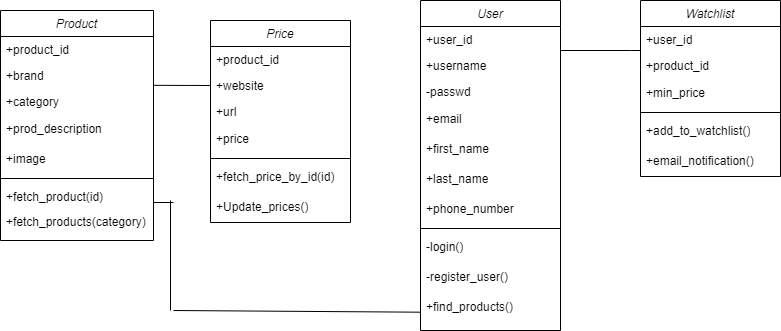
\includegraphics[width=450pt]{ClassDiagram.drawio.png}}
			\caption{Class Diagram}
			\label{fig:class-dig}
		\end{figure}
	\end{center} 
	\newpage
	\subsection{Sequence Diagram}
	\begin{center}
		\begin{figure}[!htbp]
			\centering
			\fbox{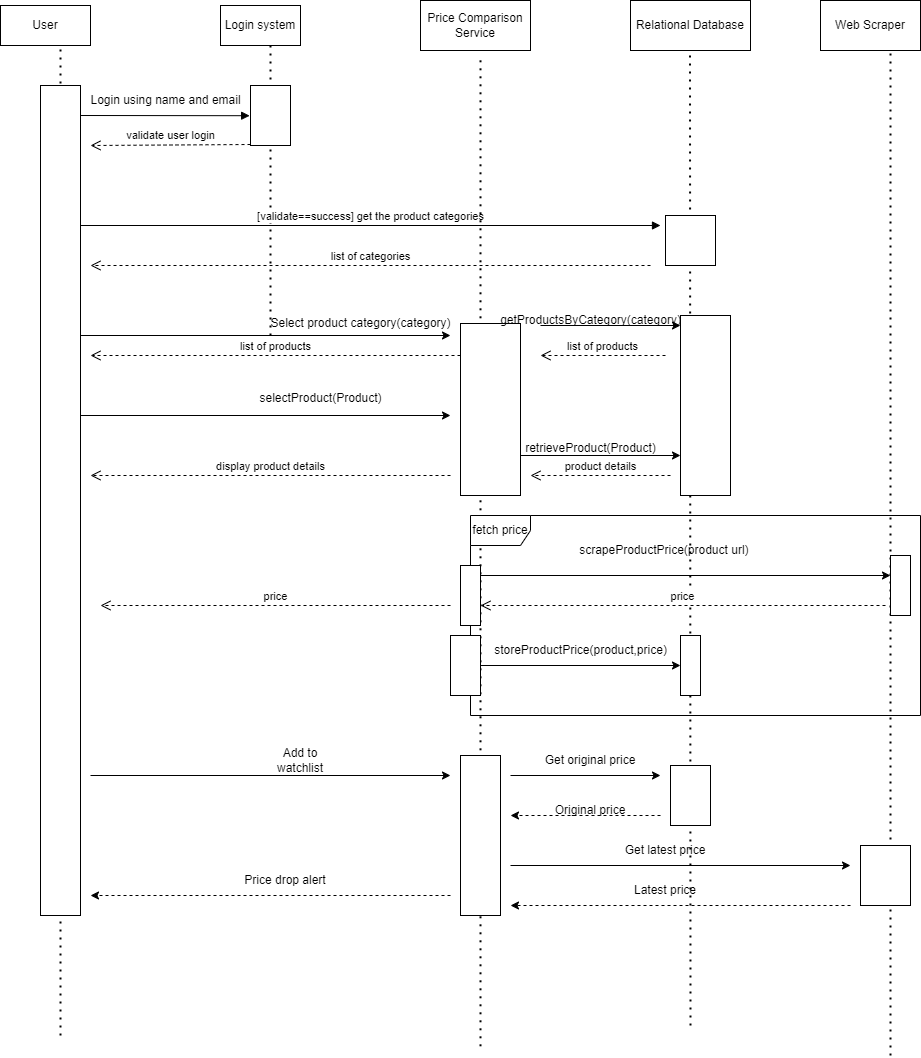
\includegraphics[width=450pt]{SequenceDiagram.drawio.png}}
			\caption{Sequence Diagram}
			\label{fig:seq-dig}
		\end{figure}
	\end{center} 
	\newpage
	\subsection{Component Diagram}
	\begin{center}
		\begin{figure}[!htbp]
			\centering
			\fbox{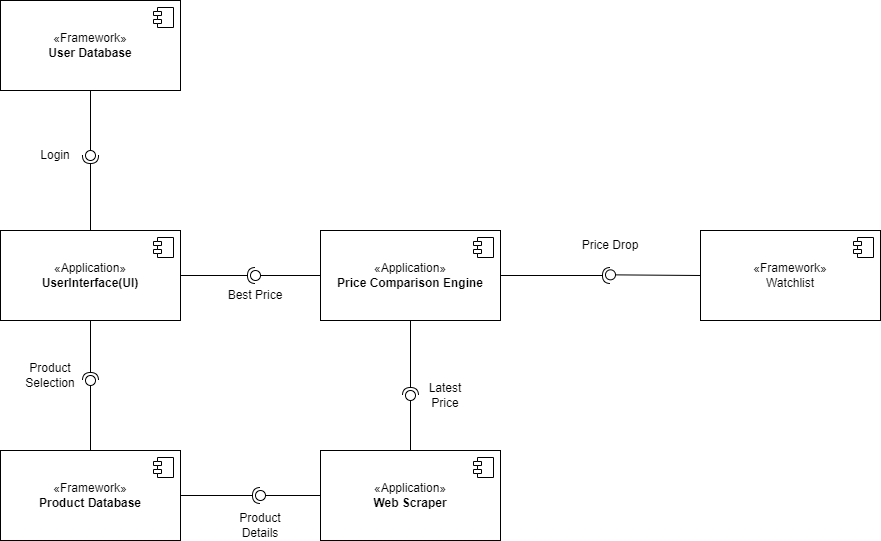
\includegraphics[width=450pt]{ComponentDiagram.drawio.png}
			}
			\caption{Component Diagram}
			\label{fig:comp-dig}
		\end{figure}
	\end{center} 
	\newpage
	\subsection{Deployment Diagram}
	\begin{center}
		\begin{figure}[!htbp]
			\centering
			\fbox{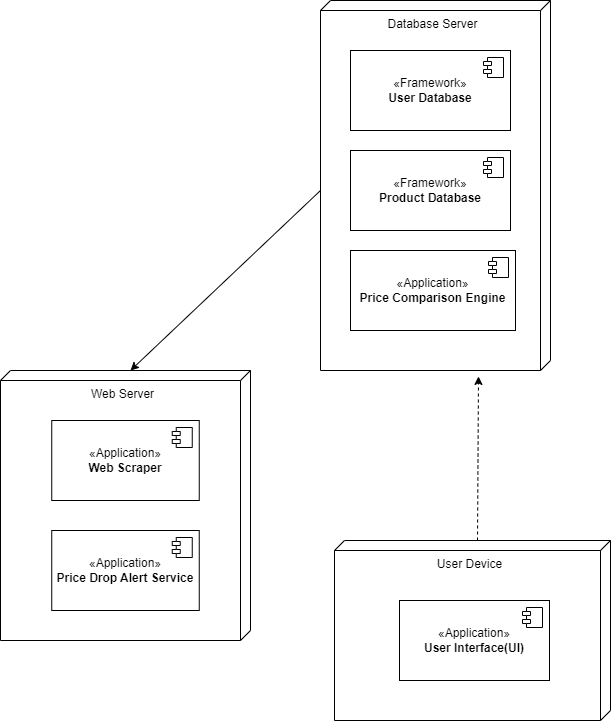
\includegraphics[width=400pt]{DeploymentDiagram.drawio.png}}
			\caption{Deployment Diagram}
			\label{fig:dep-dig}
		\end{figure}
	\end{center} 
	\newpage
	\section{Navigation Flow}
	
	\begin{center}
		\begin{figure}[!htbp]
			\centering
			\fbox{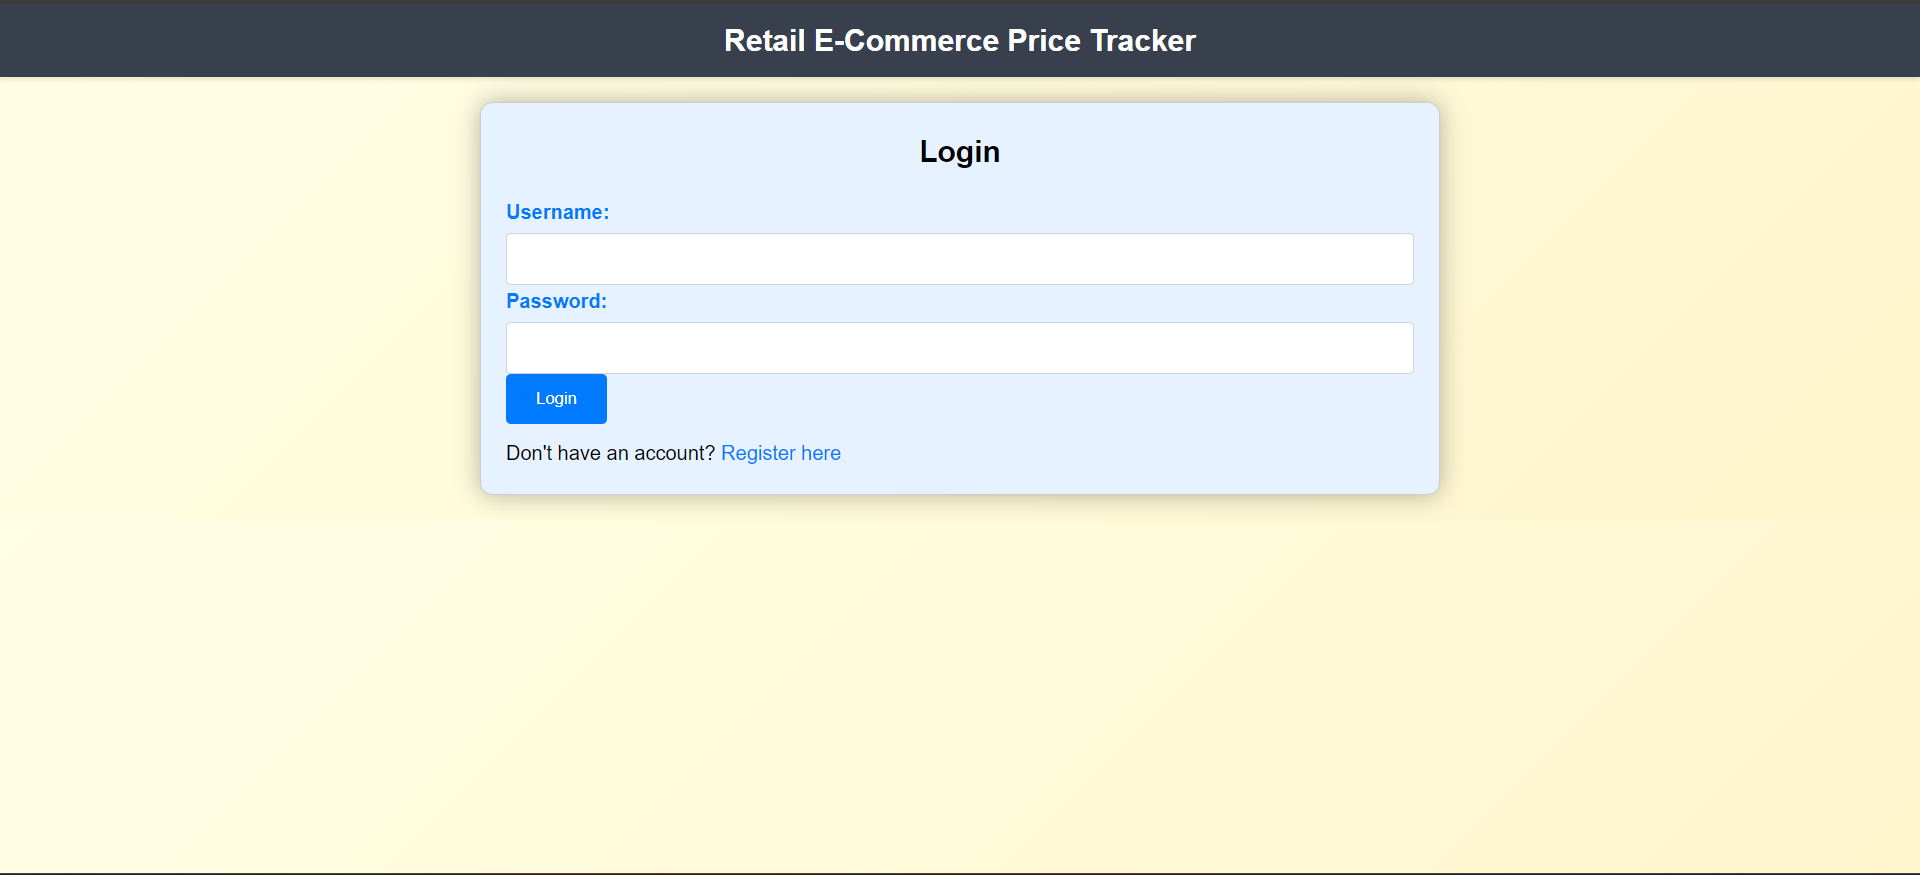
\includegraphics[width=450pt]{Login.png}}
			\caption{Login}
			\label{fig:Login}
		\end{figure}
	\end{center} 
	
	\begin{center}
		\begin{figure}[!htbp]
			\centering
			\fbox{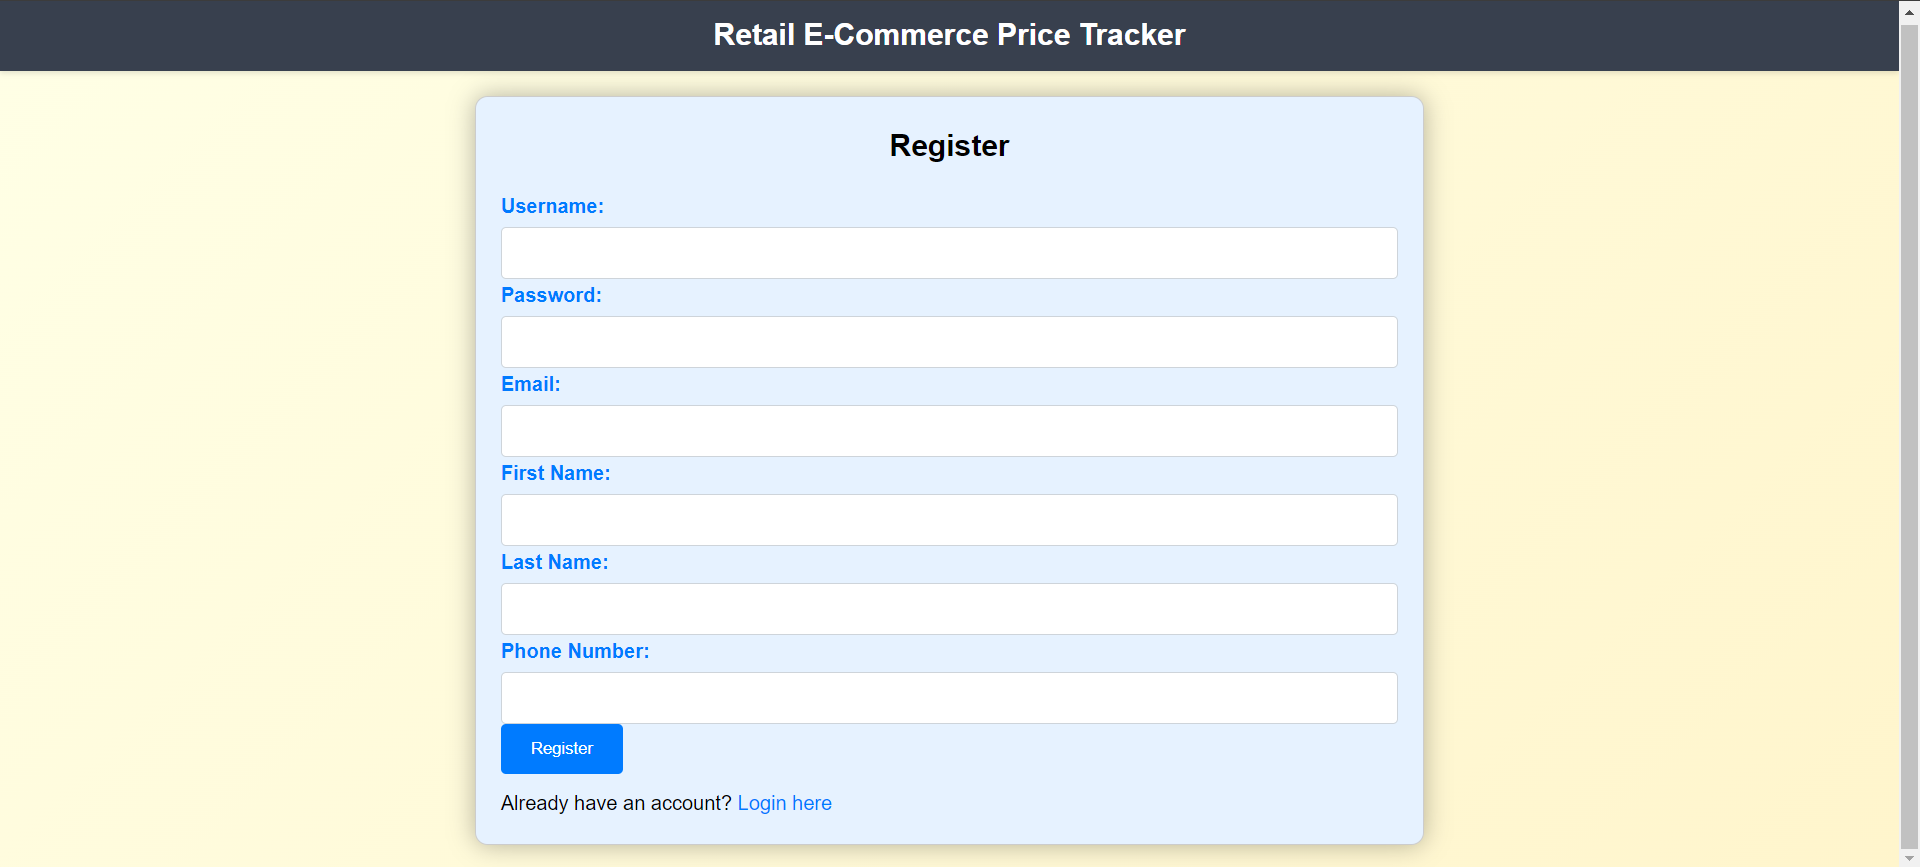
\includegraphics[width=450pt]{Registration.png}}
			\caption{Registration}
			\label{fig:Registration}
		\end{figure}
	\end{center} 
	
	\begin{center}
		\begin{figure}[!htbp]
			\centering
			\fbox{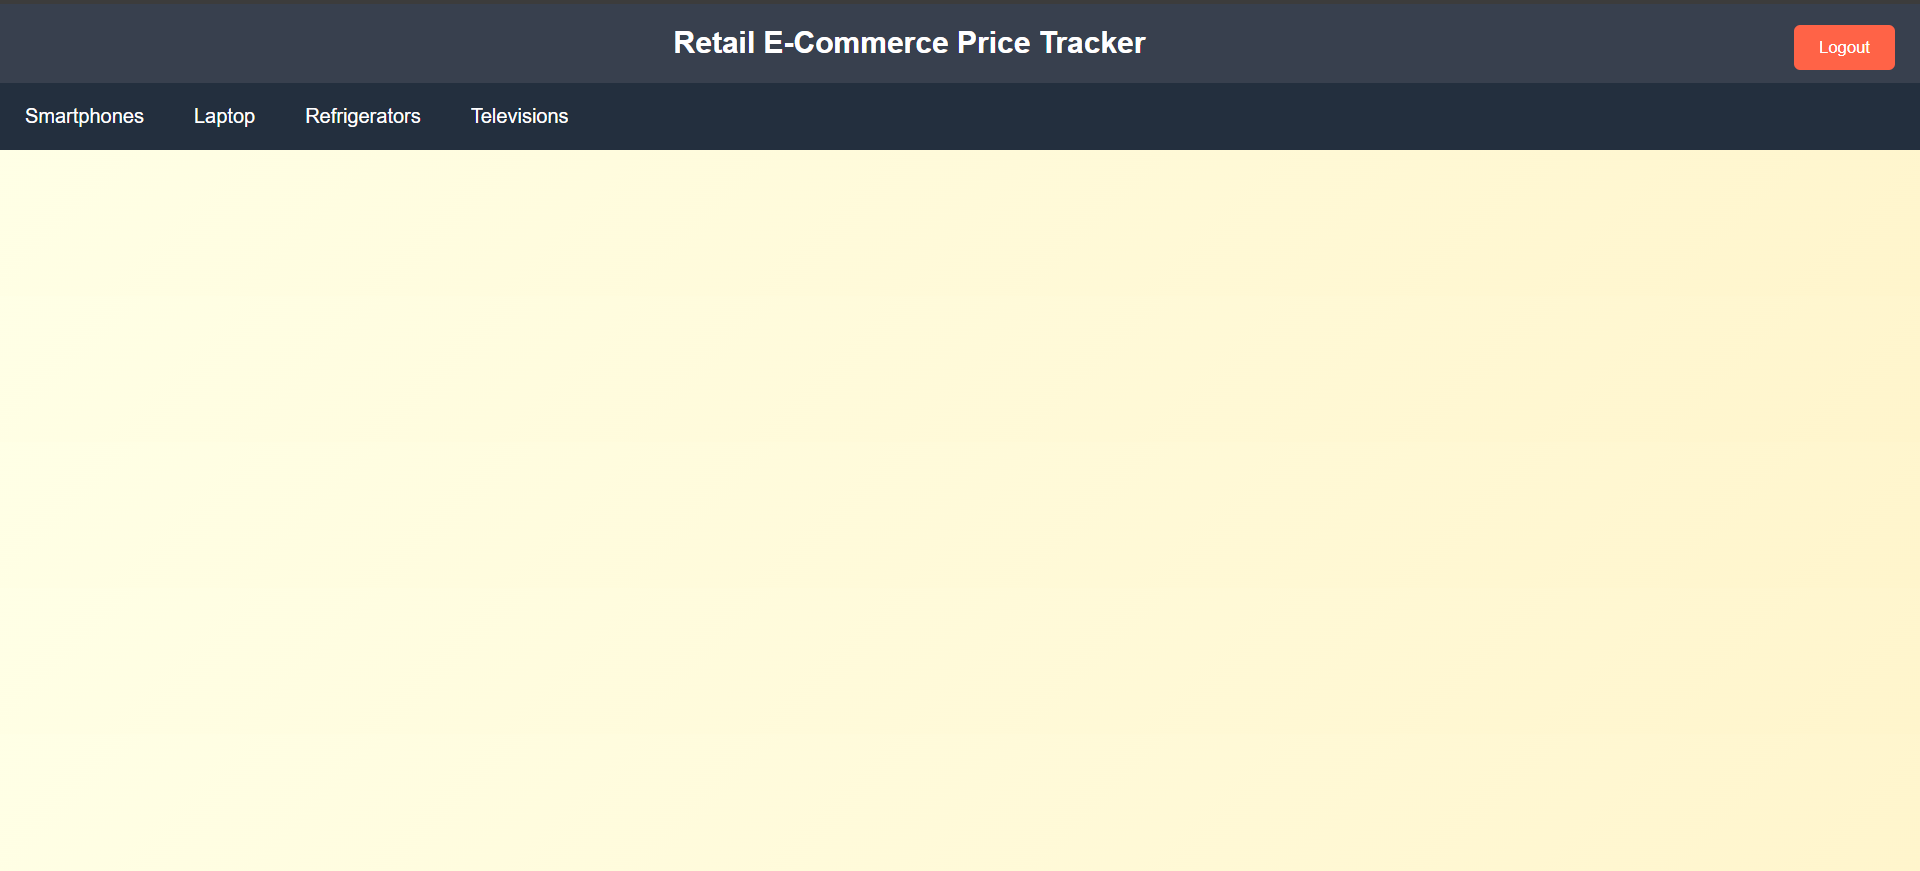
\includegraphics[width=450pt]{main1.png}}
			\caption{main1}
			\label{fig:main1}
		\end{figure}
	\end{center} 
	
	\begin{center}
		\begin{figure}[!htbp]
			\centering
			\fbox{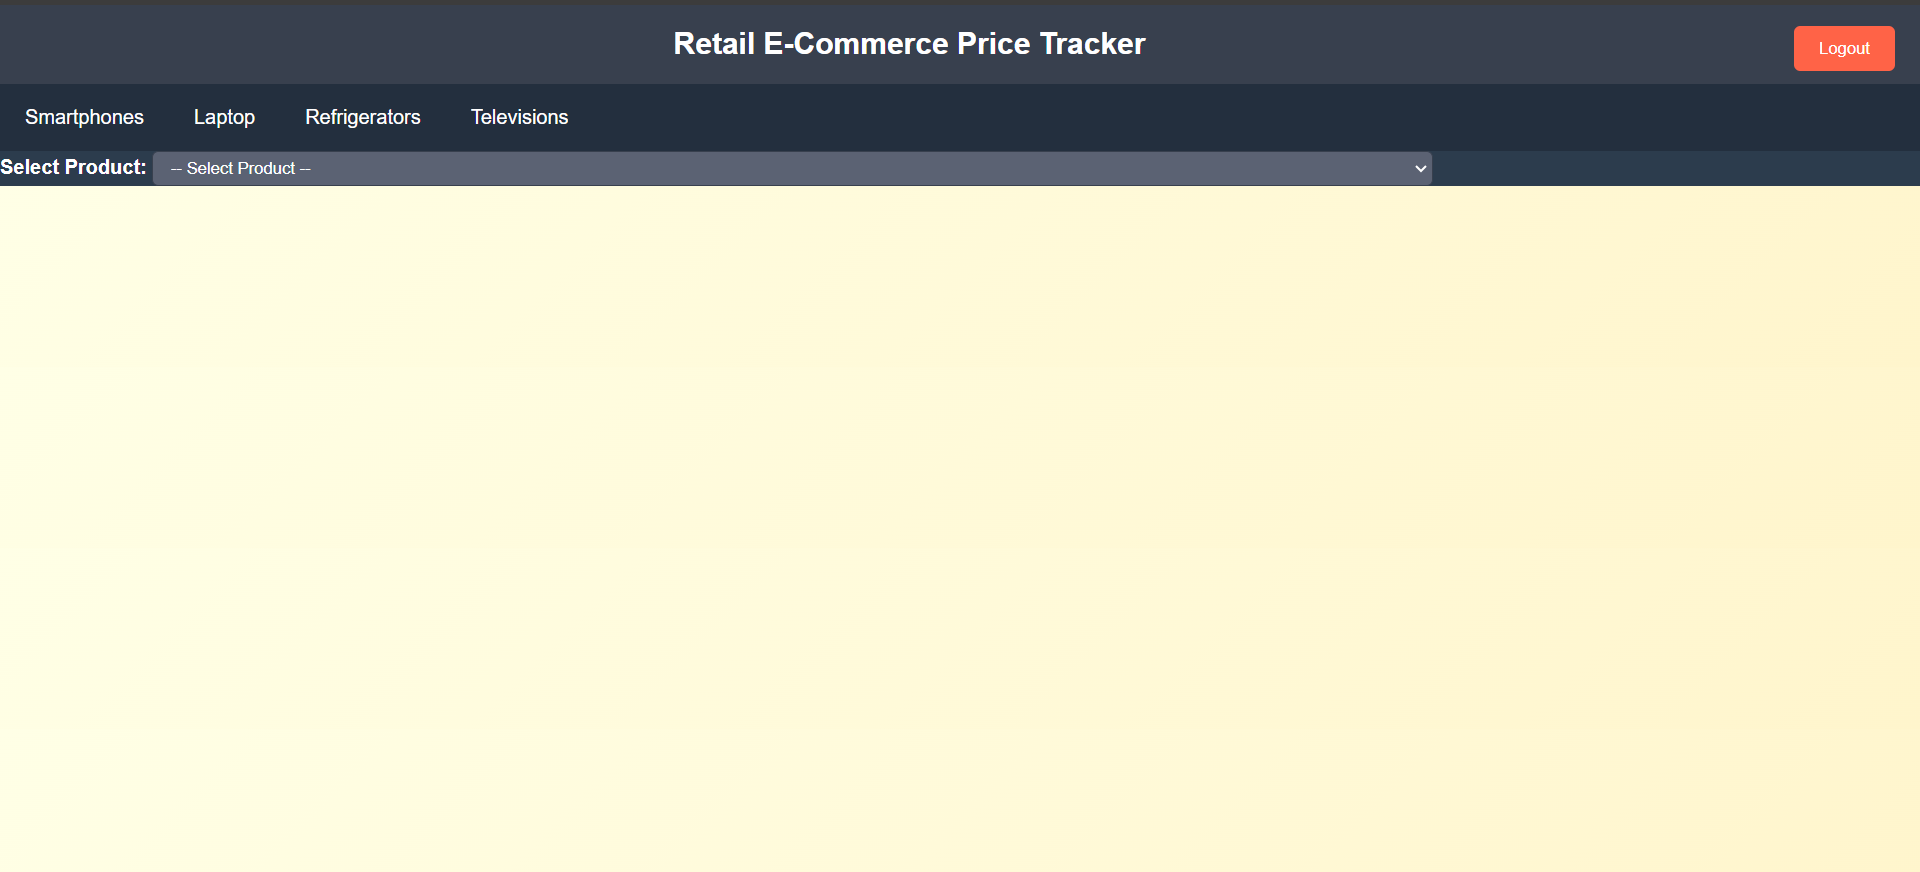
\includegraphics[width=450pt]{main2.png}}
			\caption{main2}
			\label{fig:main2}
		\end{figure}
	\end{center} 
	
	\begin{center}
		\begin{figure}[!htbp]
			\centering
			\fbox{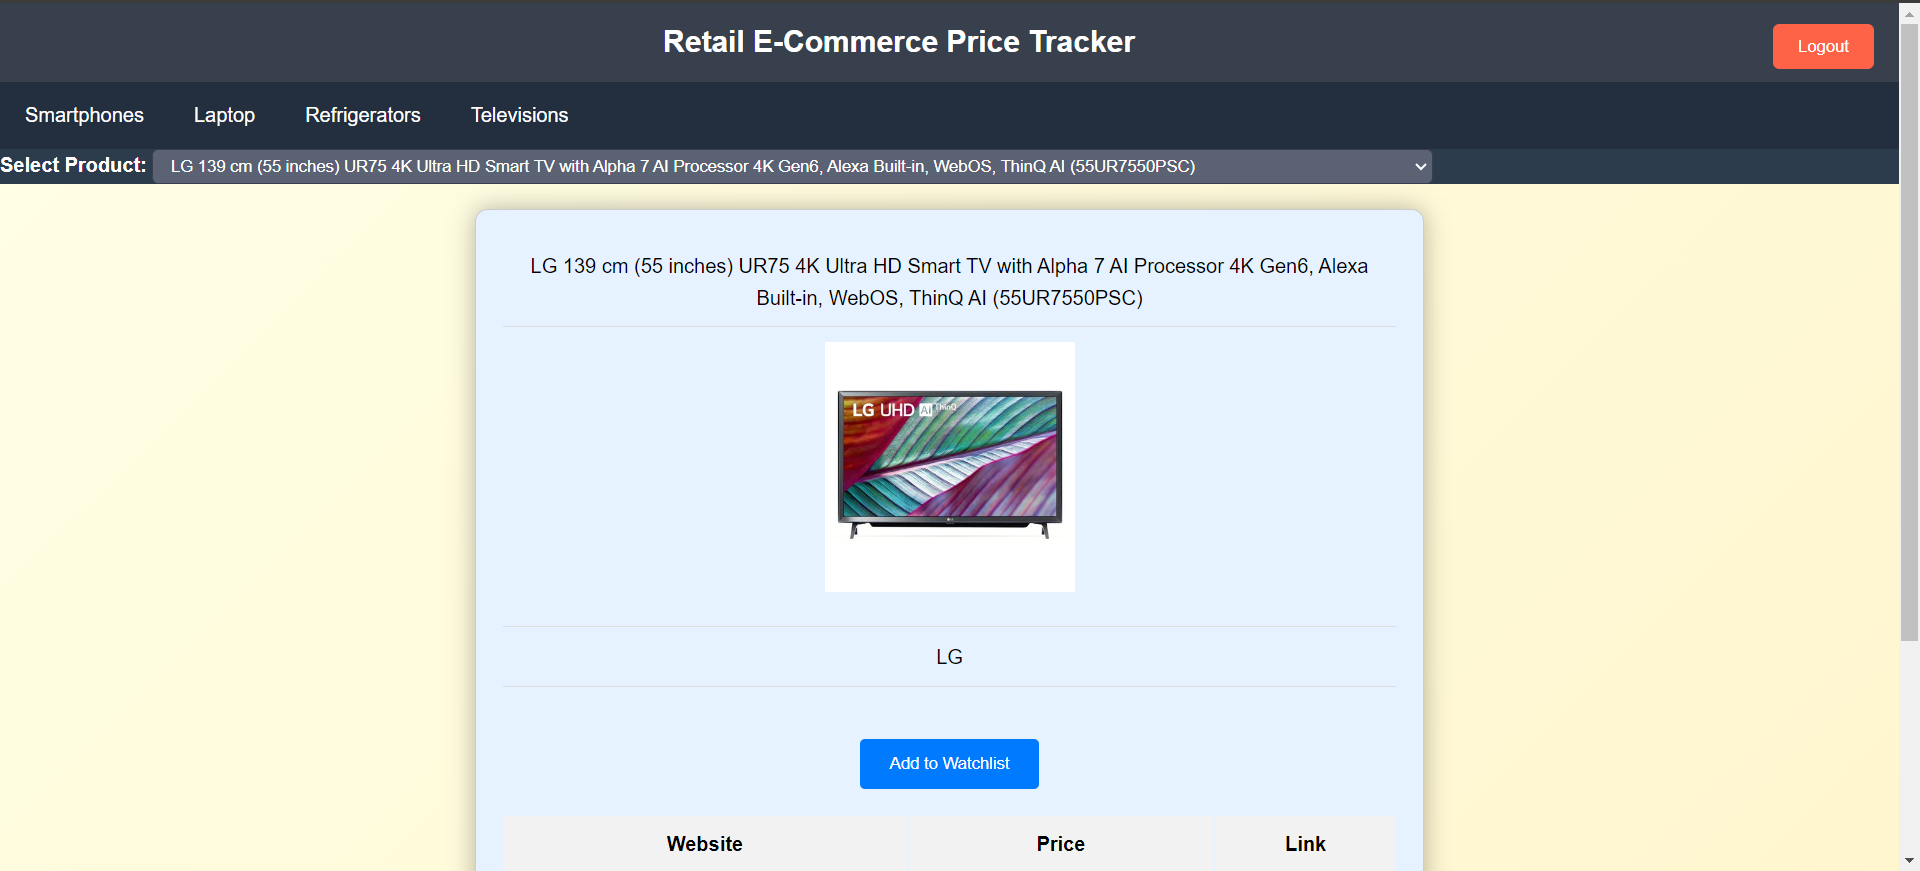
\includegraphics[width=450pt]{main3.png}}
			\caption{main3}
			\label{fig:main3}
		\end{figure}
	\end{center} 
	
	\begin{center}
		\begin{figure}[!htbp]
			\centering
			\fbox{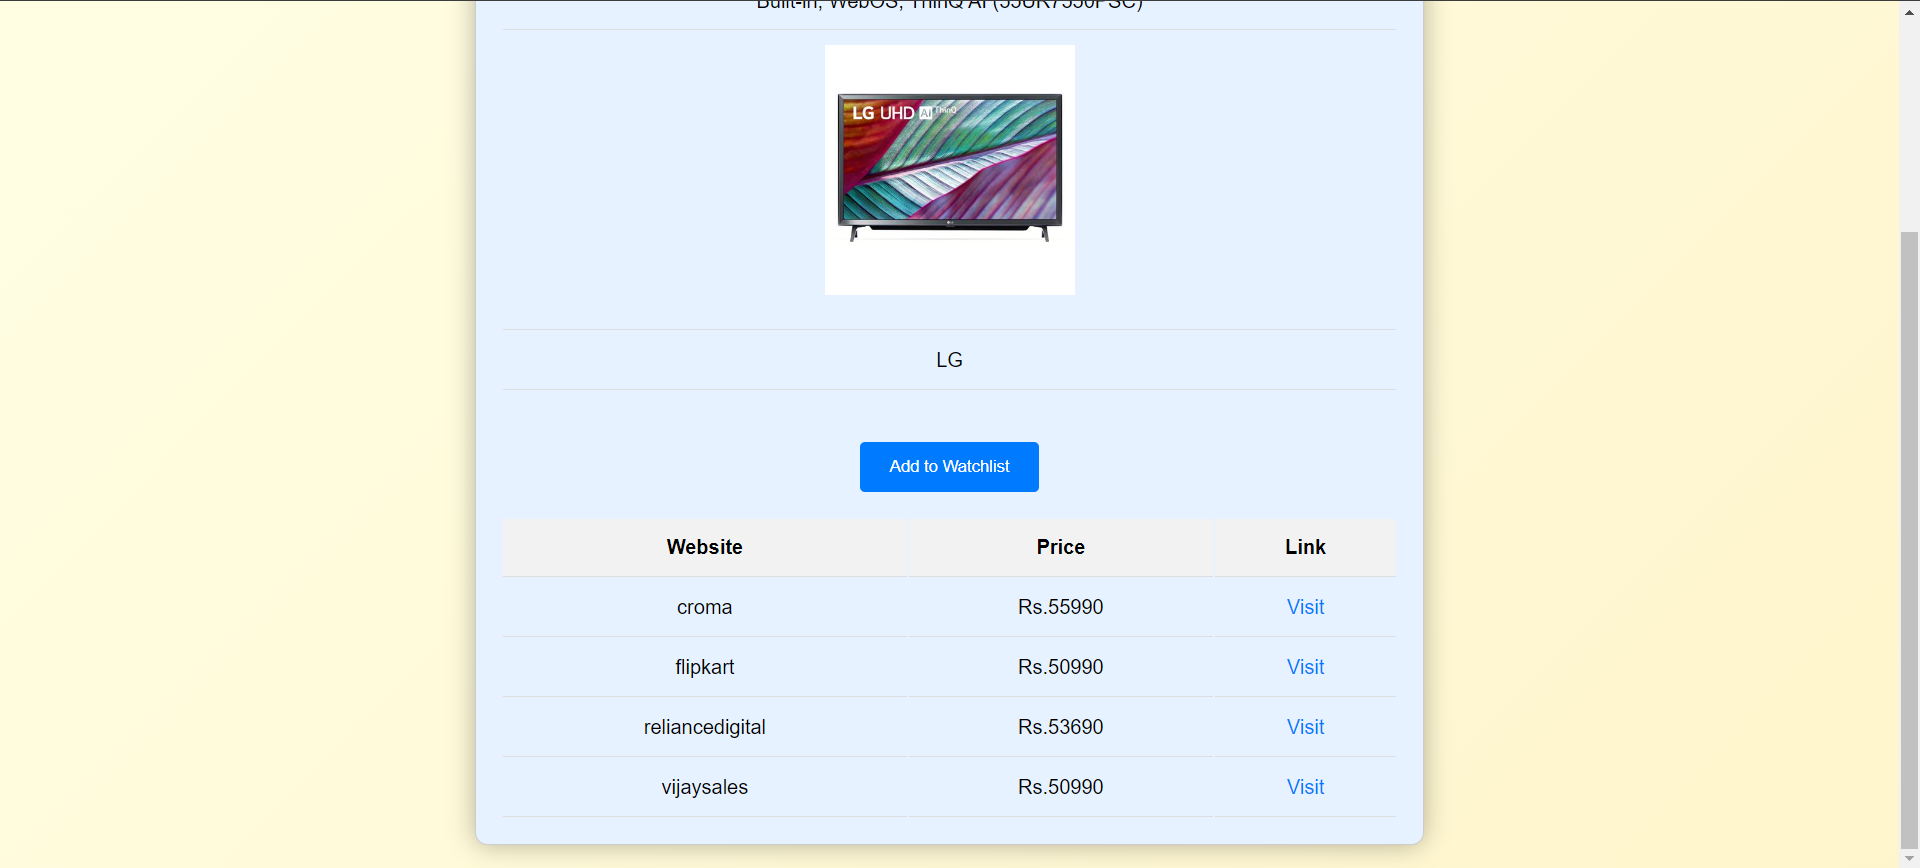
\includegraphics[width=450pt]{main4.png}}
			\caption{main4}
			\label{fig:main4}
		\end{figure}
	\end{center}
	
	\begin{center}
		\begin{figure}[!htbp]
			\centering
			\fbox{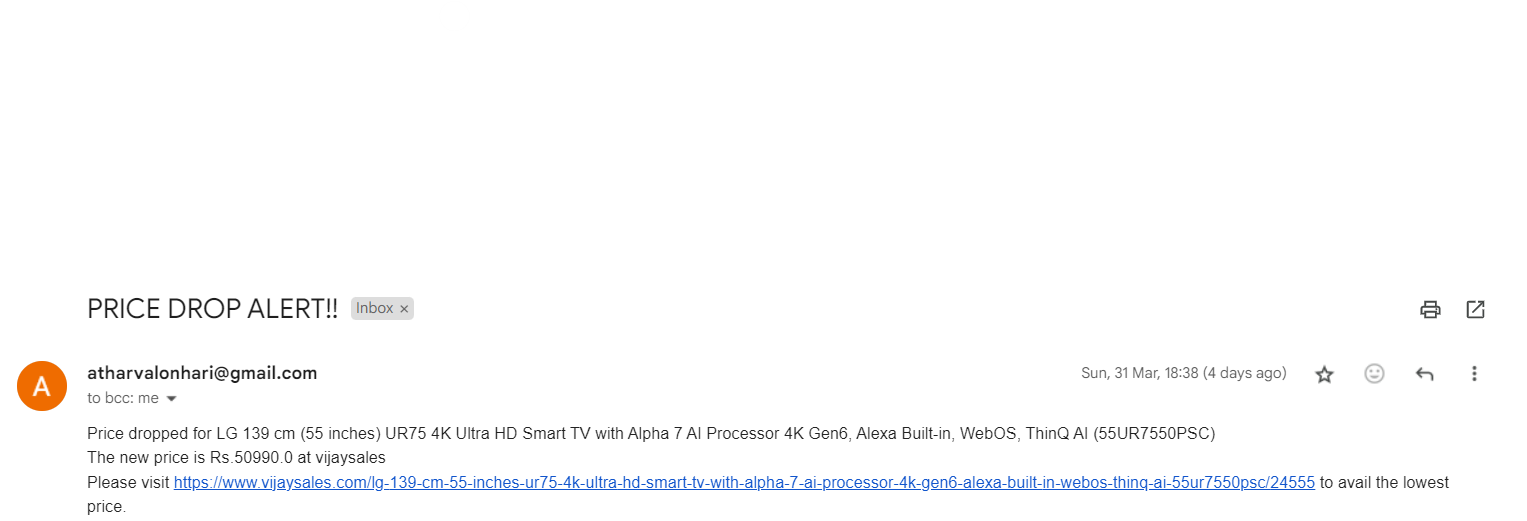
\includegraphics[width=450pt]{Pricedrop_email.png}}
			\caption{pricedrop email}
			\label{fig:pricedrop email}
		\end{figure}
	\end{center}
	
	\chapter{Summary and Conclusion}
	The Retail E-Commerce Price Tracker project aims to develop a comprehensive web application that empowers users to track and compare prices of electronic items across multiple online retailers. By leveraging web scraping techniques, the application collects real-time pricing data and presents it through a user-friendly interface, enabling users to make informed purchasing decisions and maximize savings. Key features include price comparison, price tracking with alerts, deal discovery, historical price analysis, product research, budget planning, and market analysis.
	\\
	\\
	Throughout the development process, careful consideration is given to factors such as data accuracy, legal compliance, user privacy, and system performance. Responsibilities of developers include requirements analysis, system design, coding, testing, documentation, and collaboration with stakeholders. The project estimates include time, cost, resource allocation, risk assessment, and contingency planning to ensure successful project execution.
	\\
	\\
	Use cases demonstrate the diverse applications of the Retail E-Commerce Price Tracker application for both consumers and businesses in navigating the electronic marketplace effectively. Data object descriptions outline the key entities involved in the application, including users, products, prices, and watchlists. These entities facilitate the management of user accounts, product details, pricing information, and price tracking functionality within the application.
	\\
	\\
	In conclusion, the Retail E-Commerce Price Tracker project aims to address the challenges faced by consumers in the electronic marketplace by providing a centralized platform for price comparison, tracking, and analysis. By empowering users with real-time pricing data and personalized tools, the application facilitates informed decision-making and enhances the overall shopping experience. Through continuous improvement and adaptation to user feedback, the Electronic Price Tracker application strives to remain a valuable resource for consumers and businesses alike in the dynamic landscape of online retail.
	\end{document}\end{document}			% End of Report
